%%%Variables

%%%
\question An ideal gas consists of $N$ many diatomic molecules. Because the interatomic bond resembles a spring, we model each molecule as two equal-mass balls (of mass $m$) connected by a spring.

The motion of each molecule consists of:
\begin{itemize}
	\item Momentum of the center of mass (translational momentum) in 3 dimensions: $\vec{p}_{trans}=p_x\hat{x}+p_y\hat{y}+p_z\hat{z}$
	\item Vibrational momentum relative to the center of mass in one dimension $p_{rel}$. Note that the two masses do not vibrate independently, but instead can be treated as a single particle with mass $\mu=m_1m_2/(m_1+m_2)=\frac{1}{2}m$ with momentum $p_{rel}$.
	\item Associated with the vibrational motion is the stretching and squeezing of the interatomic spring. Assume the spring has a spring constant $k_s$ (not to be confused with Boltzmann's constant!) and an equilibrium length $r_0$.
	\item Finally, the molecule is able to rotate in two directions with angular speeds $\omega_x$ and $\omega_z$ (the molecule is symmetric about the $y$ axis, so rotations about this axis don't contribute to the molecule's energy.) The moment of inertia about the $x$ and $z$ axis is the same; just call it $I$.
\end{itemize}
This motion is sketched in the figure below:
\begin{figure}[ht!]
	\centering
\begin{tabular}{cc}
	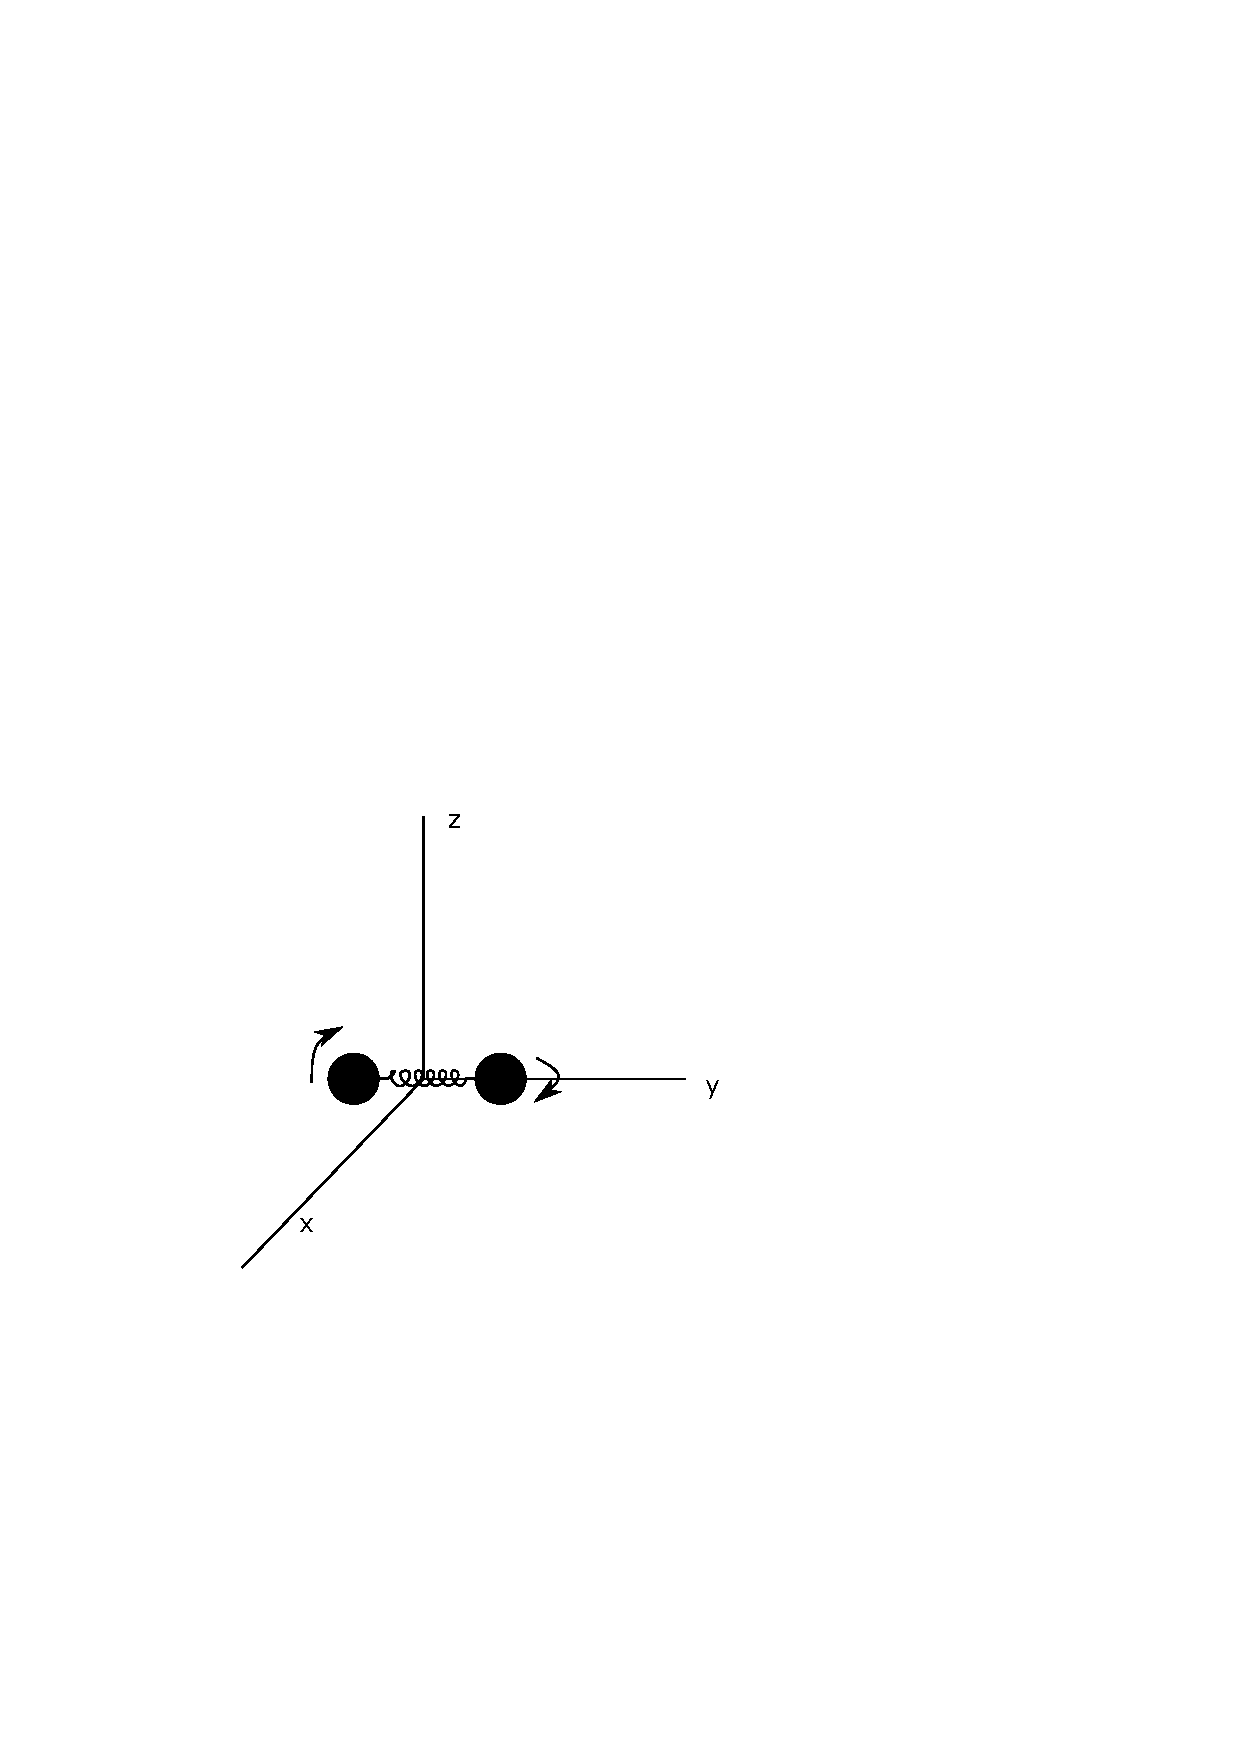
\includegraphics[width=5cm]{diatomic1} & 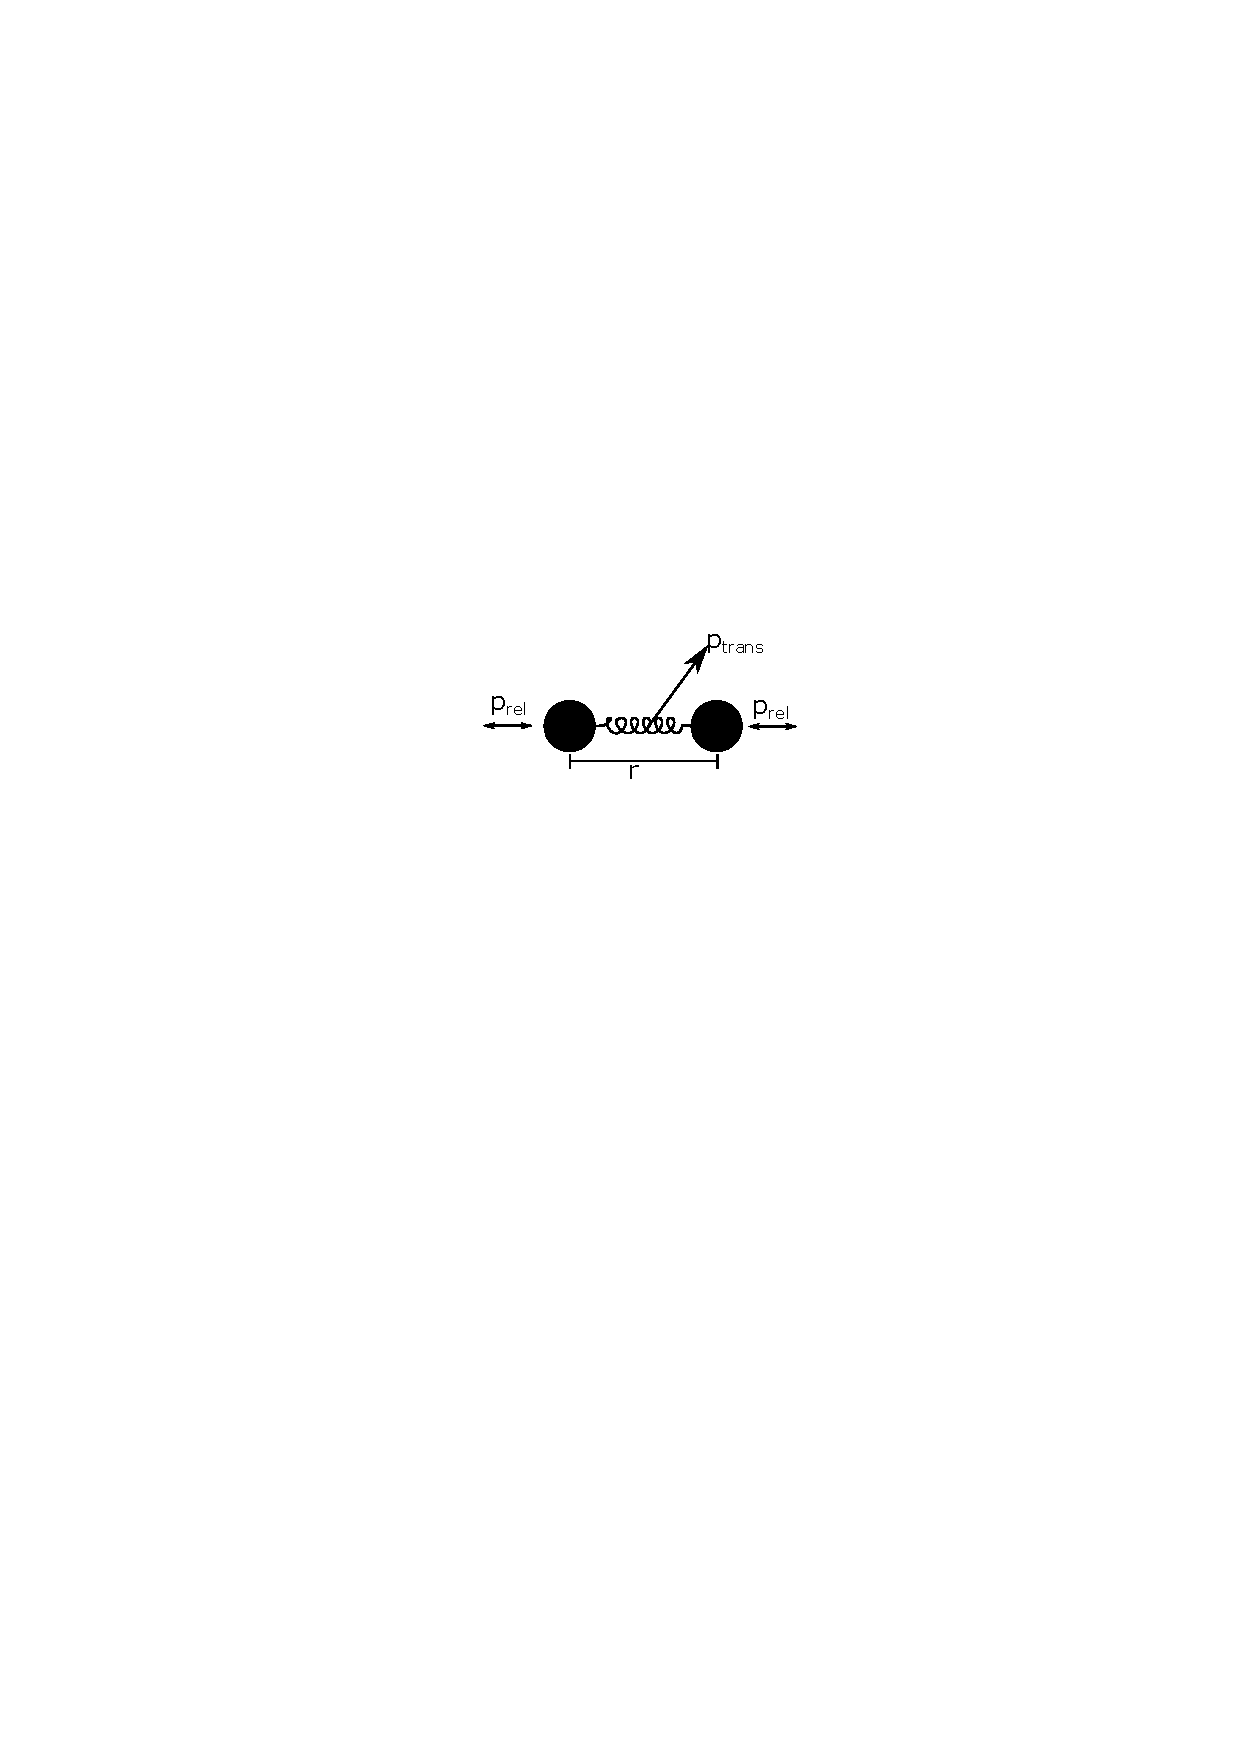
\includegraphics[width=5cm]{diatomic2}
\end{tabular}
\end{figure}

\begin{parts}
	\part In terms of the variables defined above, what is the total energy (the Hamiltonian) of each molecule?
	\vspace{2cm}
	\part If the gas is in equilibrium at some temperature $T$, what is the total  (average) internal energy of the gas (in terms of Boltzmann's constant $k_B$ and the temperature $T$)?
	\vspace{2cm}
	\part If the temperature is 300 K, and the molecule is a nitrogen $N_2$ molecule (each atom is a nitrogen atom with a mass $m=14$ amu $\approx 2.3\times10^{-26}$ kg ), what is the ``root mean square'' speed $v_{rms}=\sqrt{\left<v^2\right>}$?
\end{parts}